\documentclass[12pt]{article}
\pagestyle{plain}
\usepackage{graphicx}
\usepackage{float}
\usepackage[spanish]{babel}
\usepackage [utf8]{inputenc}
\usepackage{verbatim}

\begin{document}

\tableofcontents
\clearpage

\section{Hipótesis y Aclaraciones}

Si al comando Mover se le pasa como destino un directorio, deberá mover a éste el archivo de origen con su mismo nombre.

En los directorios utilizados para archivos de datos (\verb|$DATADIR| y sus subdirectorios), no deben existir archivos ordinarios con el nombre "dup", ya que no permitiría la creación de secuencias de duplicados (para lo cual \verb|dup| deber ser un directorio). En rigor de verdad esta situación podrí­a manejarse, ya sea eliminando los archivos ordinarios de nombre "dup" para crear directorios en su lugar, o descartando los archivos duplicados. Consideramos que no es correcto no almacenar los duplicados, y además no es necesario tener archivos de nombre "dup", debido a que los archivos de entrada tienen nombres con estructuras definidas que no permiten a "dup" ser un archivo de entrada válido.

La correcta inicialización del entorno queda indicada mediante una variable definida a tal propósito (\verb|$ENTORNO_INICIALIZADO|). Basta con chequear desde un comando la existencia de esta variable para asumir un entorno de trabajo válido.

La ruta relativa de \verb|practico.conf| respecto del comando iniciar debe ser: \verb|../conf/practico.conf|. De esta forma se asegura que iniciar pueda encontrarlo y a partir de él recibir cualquier otra información sobre rutas que necesite para continuar su correcta ejecución.

En el interprete la validación de que no haya archivos repetidos, se realiza verificando que los nombres no sean iguales y los contenidos tampoco. También como el enunciado pide que para los archivos de contratos generados se mantenga un formato numérico de diez caracteres para la parte entera y dos caracteres para la parte decimal, en caso de existir un número que tenga màs de esos caracteres (ya que puede suceder, al haber archivos cuyos registros tienen campos numéricos de hasta dieciseis caracteres para la parte entera) para la parte entera se cortarán los primeros diez caracteres de izquierda a derecha y para la decimal se cortarán los primeros dos caracteres de izquierda a derecha del número en cuestión.

DETALLAR HIPÓTESIS ASUMIDAS SOBRE LA ESTRUCTURA DE DIRECTORIOS PARA PERMITIR A INSTALAR ENCONTRAR \verb|practico.conf|.

\section{Problemas relevantes}

Quizas no haya sido un problema relevante pero si una cuestión que nos demando un poco de trabajo el tema de manejar números decimales con ',' como separador en vez de '.' ya que tanto bash como perl toman los números de punto flotante con un '.' como separador, con lo cual hubo que hacer manejos para poder mantener una cierta coherencia con lo que pedia el enunciado y el lenguaje.

DETALLAR PROBLEMAS ENCONTRADOS DURANTE EL DESARROLLO Y LAS PRUEBAS.



\section{Archivo README: Instructivo de instalación}
Cuando esté terminado el README insertar en el \verb|.tex| según su ruta haciendo:
\begin{verbatim}
\verbatiminput{ruta/README}
\end{verbatim}

\section{Comandos Desarrollados}
\subsection{Comando Mover}
\begin{description}
	\item [Tipo de comando:] Solicitado
	
	\item [Archivos de entrada:] Archivo especificado por el parámetro 1
	
	\item [Archivos de salida:] Archivo o directorio especificado por el parámetro 2; archivo de log del comando que lo invoca: \verb|$LOGDIR/comando.log|
	
	\item [Parámetros:]
	\begin{enumerate}
		\item Archivo de origen a mover
		\item Archivo o directorio de destino
		\item (Opc.) Comando que invoca a mover, permite guardar información en su log
	\end{enumerate}
	
	\item [Ejemplos de invocación:]
	Sea \verb|a1| la ruta a un archivo existente, \verb|d1| un directorio existente, invocando como:
	\begin{verbatim}$ mover a1 d1\end{verbatim}
	el comando mueve el archivo a1 al directorio \verb|d2|, informando que la operación es exitosa. Por mover se entiende que cambia el directorio padre del archivo origen.\\
	Sea \verb|a1| un archivo existente, \verb|d2| una ruta inválida, invocando como:
	\begin{verbatim}$ mover a1 d2\end{verbatim}
	el comando \verb|mv|, invocado por mover, informa que el directorio de destino no existe.\\
	Sea \verb|a1| y \verb|ruta/a2| archivos existentes, donde \verb|ruta/dup| no existe, invocando como:
	\begin{verbatim}$ mover a1 ruta/a2\end{verbatim}
	el comando crea en ruta el subdirectorio \verb|dup|, y mueve allí­ el archivo \verb|a1| con nombre \verb|a2.1|. Este representa el primer duplicado de \verb|a2|. Si se vuelve a invocar como:
	\begin{verbatim}$ mover ax ruta/a2\end{verbatim}
	el comando mueve \verb|ax| a \verb|ruta/dup/a2.2|. Así­ va formando una secuencia de archivos duplicados para no permitir la sobreescritura.\\
	Sea \verb|a1| un archivo existente, \verb|ruta/a1| otro archivo existente, invocando como:
	\begin{verbatim}$ mover a1 ruta\end{verbatim}
	el comando intenta mover \verb|a1| a \verb|ruta/a1|; al existir este archivo, se añade un duplicado a la secuencia de \verb|a1| (o se la inicia si no existen duplicados previos).\\
	Sea \verb|a3| una ruta inválida, \verb|a4| una ruta válida o inválida, invocando como:
	\begin{verbatim}$ mover a3 a4 com1\end{verbatim}
	el comando informa que el archivo de origen es inexistente. Además, por haber incluído el tercer parámetro, el comando guarda en \verb|$LOGDIR/com1.log|, a través del comando \verb|glog| todos los mensajes de información y/o error que, al igual que en las demás ejecuciones, también envía por la salida estándar.
	
	\item [Código fuente:]
\end{description}
{\footnotesize
\verbatiminput{../bin/mover}
}

\subsection{Comando Instalar}
\begin{description}
	\item [Tipo de comando:] Solicitado
	
	\item [Archivos de entrada:] 
		El archivo de configuración, si es que existe, para una instalación anterior. Se encuentra en:
		\begin{verbatim}
			$grupo/conf/practico.conf
		\end{verbatim}
		Todos los archivos binarios y de datos que seran instalados, se encuentran en 
		\begin{verbatim}
			$grupo/inst/bin/ 
		\end{verbatim}	
		y 
		\begin{verbatim}	
			$grupo/inst/data/
		\end{verbatim}
	
	
	\item [Archivos de salida:] 
		\begin{itemize}
			\item	Un archivo de configuración que se generará a partir de la instalación. Se encontrará en  
					\begin{verbatim}	
						$grupo/conf/practico.conf
					\end{verbatim}	
			\item Todos los archivos binarios y de datos que serán instalados. Se encontrarán en 
					\begin{verbatim}	
						$BINDIR 
					\end{verbatim}
					y 
					\begin{verbatim}	
						$DATADIR.
					\end{verbatim}
					
			\item	Un archivo de log que tenga toda la información de registro de la instalación. Se encuentra en 
					\begin{verbatim}
						$grupo/log/instalar.log
					\end{verbatim}
					
			\item	Un directorio donde se alojaran los archivos de log de todos los componentes que se ejecuten. Se encontrará en 
					\begin{verbatim}
						$LOGDIR.
					\end{verbatim}
		\end{itemize}
	
	\item [Hipotesis:] 
			Para la instalación de los componentes necesarios, estos deben encontrarse dentro del directorio:
				\begin{verbatim}
					$grupo/inst/bin
				\end{verbatim}
			Todos los archivos que se encuentren en ese directorio se consideraran como componentes a instalar. 
			El instalador detecta una instalación previa en caso de que encuentre su respectivo archivo de configuración. 
			En caso de encontrar un componente imprime por pantalla que se ha encontrado ese componente y no se instalará.
	
	
	\item [Ejemplos de invocación:]
		\begin{verbatim}
			$ instalar
		\end{verbatim}
		
		De esta forma se inicia la instalacion del sistema.
	
	\item [Código fuente:]
\end{description}


\subsection{Comando Iniciar}
\begin{description}
	\item [Tipo de comando:] Solicitado
	
	\item [Archivos de entrada:] El archivo de configuración \verb|practico.conf|
	
	\item [Archivos de salida:] El archivo de log \verb|$LOGDIR/iniciar.log|
	
	\item [Ejemplo de invocación:] El comando iniciar debe invocarse como
	\begin{verbatim}$ . iniciar\end{verbatim}
	El comando chequeará la presencia en el archivo de configuración \verb|practico.conf| de las variables indispensables para el correcto funcionamiento de todos los comandos. Solicitará parámetros necesarios para el comando detectar: cantidad máxima de ciclos de ejecución y tiempo de espera entre ciclos, expresado en minutos. También dará la posibilidad de ejecutar detectar a continuación, o bien recibir indicaciones de cómo hacerlo manualmente. La ejecución de este comando deja inicializado el entorno de trabajo para la sesión de bash actual. Cualquier otra sesión de bash en que se quieran utilizar los comandos del trabajo, no representará un entorno válido si no se ejecuta en ella el comando iniciar.
	
	\item [Código fuente:]
\end{description}
{\footnotesize
\verbatiminput{../bin/iniciar}
}

\subsection{Comando Detectar}
\begin{description}
	\item [Tipo de comando:] Solicitado
	
	\item [Archivos de entrada:] Archivos ubicados en el directorio \verb|$DATADIR|
	
	\item [Archivos de salida:] Archivos de \verb|$DATADIR| que cumplen con el criterio de validez de nombres
	
	\item [Ejemplos de invocación:]	El comando solo puede invocarse como
	\begin{verbatim}$ detectar\end{verbatim}
	de esta manera, lo que hace es verificar la validez de los archivos ubicados en el directorio \verb|$DATADIR|, para así colocar los correctos como archivos de entrada del intérprete en \verb|$DATADIR/ok|, y los incorrectos en \verb|$DATADIR/nok|.
	
	\item [Código fuente:]
\end{description}
{\footnotesize
\verbatiminput{../bin/detectar}
}

\subsection{Comando Interprete}
\begin{description}
	\item [Tipo de comando:] Solicitado
	
	\item [Archivos de entrada:]
	\begin{enumerate}
		\item Archivos de Practico Recibidos en \verb|$DATADIR/ok|
		\item Tabla de Separadores \verb|$DATADIR/conf/T1.tab|
		\item Tabla de Campos \verb|$DATADIR/conf/T2.tab|
	\end{enumerate}
	
	\item [Archivos de salida:]
	\begin{enumerate}
		\item Archivo de Contratos de Préstamos Personales \verb|$DATADIR/new/CONTRAT.<pais>|
		\item Archivos (duplicados) Rechazados \verb|$DATADIR/nok/<nombre del archivo>|
		\item Archivos de Practico Procesados \verb|$DATADIR/old/<pais>-<sistema>-<año>-<mes>|
		\item Log \verb|$DATADIR/log/interprete.log|
	\end{enumerate}
	
	\item [Ejemplos de invocacin:]	El comando solo puede invocarse como
	\begin{verbatim}$ interprete\end{verbatim}
	de esta manera, lo que hace es procesar los archivos que se encuentran en el directorio \verb|$DATADIR/ok|, procesarlos y generar los archivos de contrato, con los cuales se llega a un formato estandar, denominados \verb|$DATADIR/new/CONTRAT.<pais>| en el directorio \verb|$DATADIR/new|. Los archivos ya procesados los deja en el directorio \verb|$DATADIR/old|, y los repetidos en \verb|$DATADIR/nok|.
	
	\item [Código fuente:]
\end{description}
{\footnotesize
\verbatiminput{../bin/interprete}
}

\subsection{Comando Glog}
\begin{description}
	\item [Tipo de comando:] Solicitado
	
	\item [Archivos de salida:] Los archivos correspondientes a los logs registrados. Estos archivos se encontrarán en el directorio: 
		\begin{verbatim}
			$LOGDIR
		\end{verbatim}
		%El log de la instalación se graba en el directorio fijo:
	
	\item [Parámetros:] 
		El primer parametro es de caracter obligatorio.  Indica el comando que esta generando un log.

		El segundo parametro es de caracter opcional. Indica el tipo de mensaje que puede ser informativo (I), un error severo (SE), un warning (W) o un error(E).
		
		El tercer mensaje es de caracter obligatorio. Indica el mensaje que se desea imprimir en el log.
		
	\item [Consideraciones:]
		De acuerdo a lo solicitado en el enunciado, existe un tamaño máximo para el tamaño de los archivos de logs. 
		Una vez que se supera este limite, el programa realiza un truncamiento del archivo dejando las ultimas 50 lineas.
		Pese a que es altamente improbable, podría suceder que con estas 50 lineas se supere el tamaño máximo del archivo.
		Por lo tanto, una vez que ya se ha realizado el truncamiento se verifica que el tamaño de dichas lineas no supere el tamaño máximo establecido.
		En caso de superarlo, se dejaría al archivo vacío para que recupere la consistencia.
		
	\item [Ejemplos de invocación:]
		
		Existen dos formas distintas de invocar al comando: pasandole 2 o 3 parametros.
		
		\begin{verbatim}
			glog <Comando> <Tipo de Mensaje> <Mensaje>
			glog <Comando> <Mensaje>
		\end{verbatim}
		
		Se puede observar un ejemplo de la invocación en la captura siguiente.
		
		\begin{figure}[H]
		\centering
		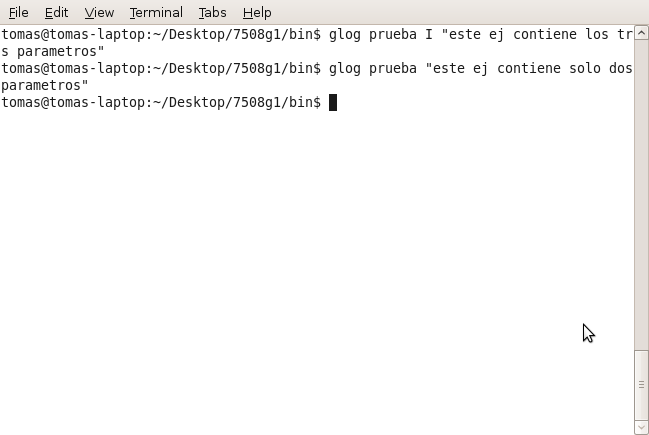
\includegraphics[scale=0.35]{imagenes/glog/01.png}
		\end{figure}
	
		Se genera un archivo llamado \emph{prueba.log} con el siguiente contenido:
	
		\begin{figure}[H]
		\centering
		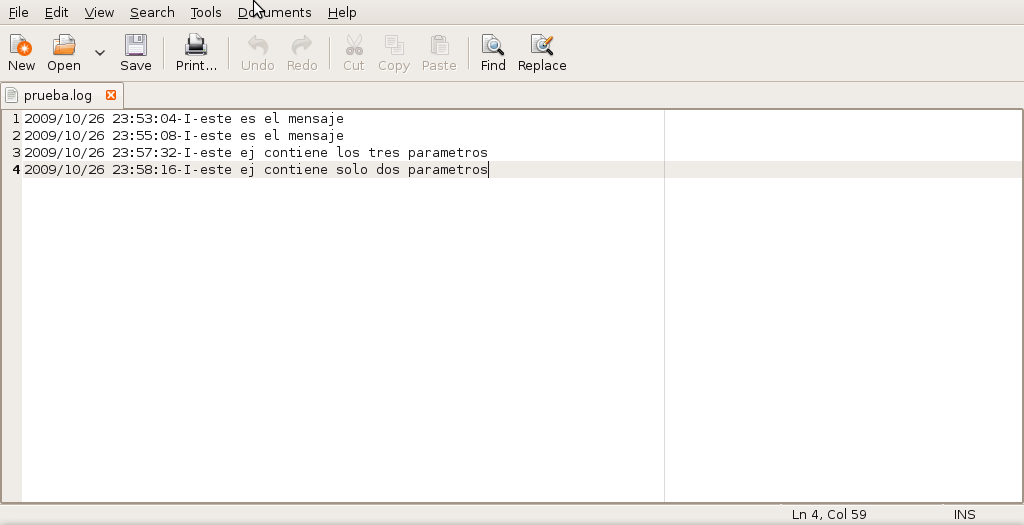
\includegraphics[scale=0.35]{imagenes/glog/02.png}
		\end{figure}
	
	
	\item [Código fuente:]
\end{description}

\subsection{Comando Vlog}
\begin{description}
	\item [Tipo de comando:] Solicitado
	
	\item [Archivos de entrada:] Archivos de log( ubicados en el LOGDIR).
	
	\item [Archivos de salida:] standar output.
	
	\item [Ejemplo de invocación:] El comando vlog puede invocarse como
	\begin{verbatim}$ vlog\end{verbatim}
        Así solo, el comando muestra por salida estandar todos los archivos de logs. 
        Obviamente esto no es lo deseable en la mayoria de los casos por lo que este comando nos ofrece varios filtros para visualizar el archivo de log de cada uno de los comandos. 
        De esta forma, se pueden filtrar los logs por comando, por fecha, hora y tipo de mensaje. 
        Cabe destacar que en la varios filtros poseen la propiedad de hacerlo por rango. 
        Por ejemplo, generalmente es bastante deseable que se filtren los sucesos que sucedieron entre tantos dias y a la vez entre un rango de horas determinadas. 
        Todo esto es posible con esta herramienta. A continuación se muestran unos ejemplos con screenshots acerca de como usarla.
        En la siguiente figura se puede ver el comando -h ( help). En ella se muestran las distintas opciones para poder filtrar los logs, y aluna opci\'on m\'as.

	\begin{figure}[H]
	\centering
	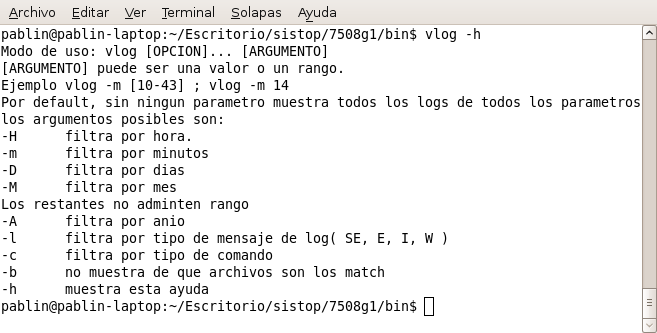
\includegraphics[scale=0.55]{imagenes/vlog/vlog_help.png}
	\caption{Help del comando vlog}
	\end{figure}

        En las posteriores figuras se puede observar el log del comando iniciar, variando la cantidad de parámetros para obtener búsquedas más precisas.

	\begin{figure}[H]
	\centering
	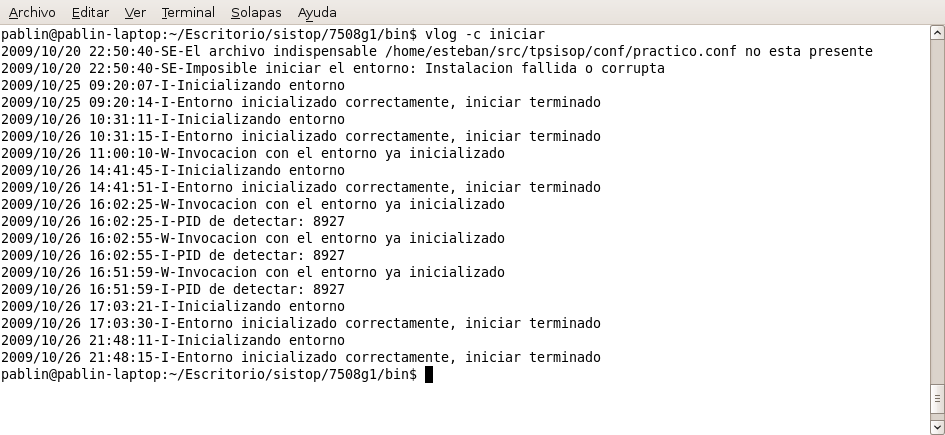
\includegraphics[scale=0.45]{imagenes/vlog/vlog_filtro_comando.png}
	\caption{vlog filtrando solo por comando(en este caso el comando iniciar)}
	\end{figure}

	\begin{figure}[H]
	\centering
	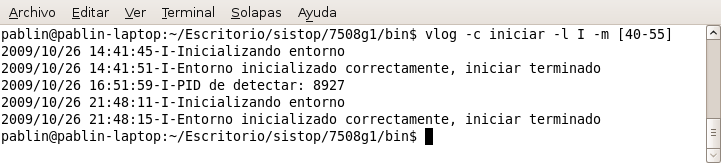
\includegraphics[scale=0.55]{imagenes/vlog/vlog_comando_Tmsj_min.png}
	\caption{vlog con filtros más exhaustivos. Filtros: comando(-c), tipo de mensaje(-l) y por rango de minutos (-m)}
	\end{figure}

	\item [Código fuente:]
\end{description}
{\footnotesize
\verbatiminput{../bin/vlog}
}

% á é í ó ú
\subsection{Comando Reporte}
\begin{description}

	\item [Tipo de comando:] Solicitado
	
	\item [Archivos de entrada:]
		\begin{enumerate}
		\item Archivo de Contratos de Préstamos Personales ubicado en \verb|$grupo/datadir/new/CONTRAT.<pais>|
		\item Archivo Maestro Préstamos Personales Impagos ubicado \\ en \verb|$grupo/datadir/mae/PPI.mae|
		\item Tabla de Paises y Sistemas ubicadas en \verb|$grupo/conf/p-s.tab|
		\end{enumerate}

	\item [Archivos de salida:] Los archivos de salida correspondientes a este comando, se generan si el usuario lo especifica. 
		\begin{enumerate}
		\item Log  \verb|$grupo/logdir/reporte.log|
		\item Listados \verb|$grupo/datadir/list/<nombre listado>.<id>|
		\item Archivo de Modificaciones de Contratos \verb|$grupo/datadir/new/MODIF.<pais>|
		\end{enumerate}

	\item [Ejemplos de invocación:]	El comando solo puede invocarse como
	\begin{verbatim}$ reporte\end{verbatim}
	de esta manera, se carga un menu interactivo en donde el usuario puede:
		\begin{enumerate}
		\item Cargar parámetros de la consulta a realizar
		\item Activar o desactivar la grabación de los listados de consulta
		\item Activar o desactivar la grabación de modificaciones de contrato
		\item Realizar la consulta en base a los parámetros ingresados por teclado
		\end{enumerate}

	\begin{figure}[H]
	\centering
	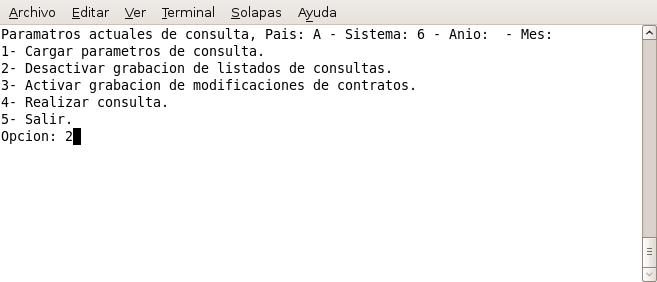
\includegraphics[scale=0.5]{imagenes/reporte/reporte_menu.png}
	\caption{Menú reporte}
	\end{figure}

	El reporte cuenta con un menú con cinco opciones disponibles, como se puede ver en la imagen anterior. 
        La carga de parámetro se realiza por teclado y el único obligatorio es el nombre del pais.
        La aplicación permite activar y desactivar la grabación de los listados y modificaciones en archivos.
        Realizar consulta impreme por pantalla los listados correspondientes y una tabla con las modificaciones. 
        En caso de haber activo la grabación en archivos, se realiza la escritura.
        La última opción, como su nombre lo indica, nos permite abandonar la aplicación.

	\begin{figure}[H]
	\centering
	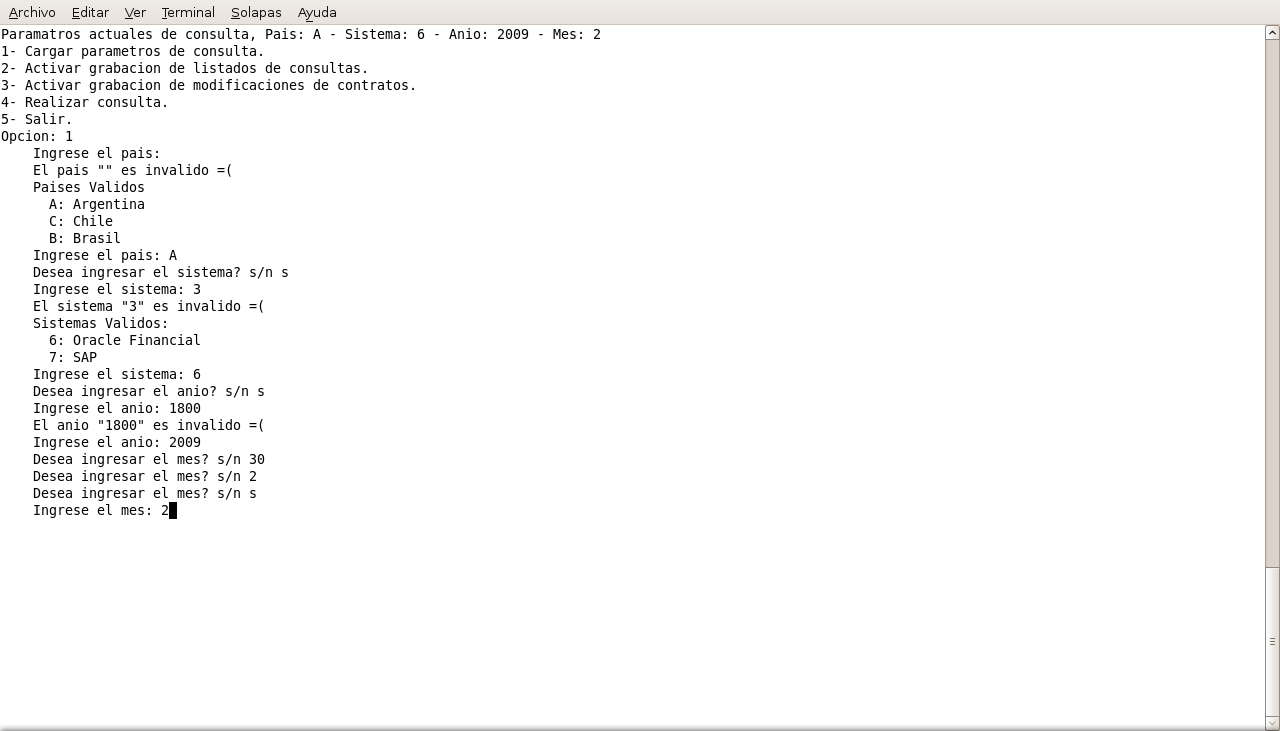
\includegraphics[scale=0.45]{imagenes/reporte/reporte_cargaParametros.png}
	\caption{Carga de parámetros}
	\end{figure}

        Esta imágen corresponde a la carga de los parámetros de consulta y a la validación de los mismos.
        En primer lugar se ingresan el pais y el sistema. 
        La validación de estos parámetros se realizar consultando la tabla de países y sistemas ubicada en \verb|$grupo/conf/p-s.tab|. 
        Luego se ingresa el año que, para superar el proceso de validación, debe ser superior a 2000. 
        Por último se ingresa el mes, el cual debe ser un número entre 1 y 12.  

	\begin{figure}[H]
	\centering
	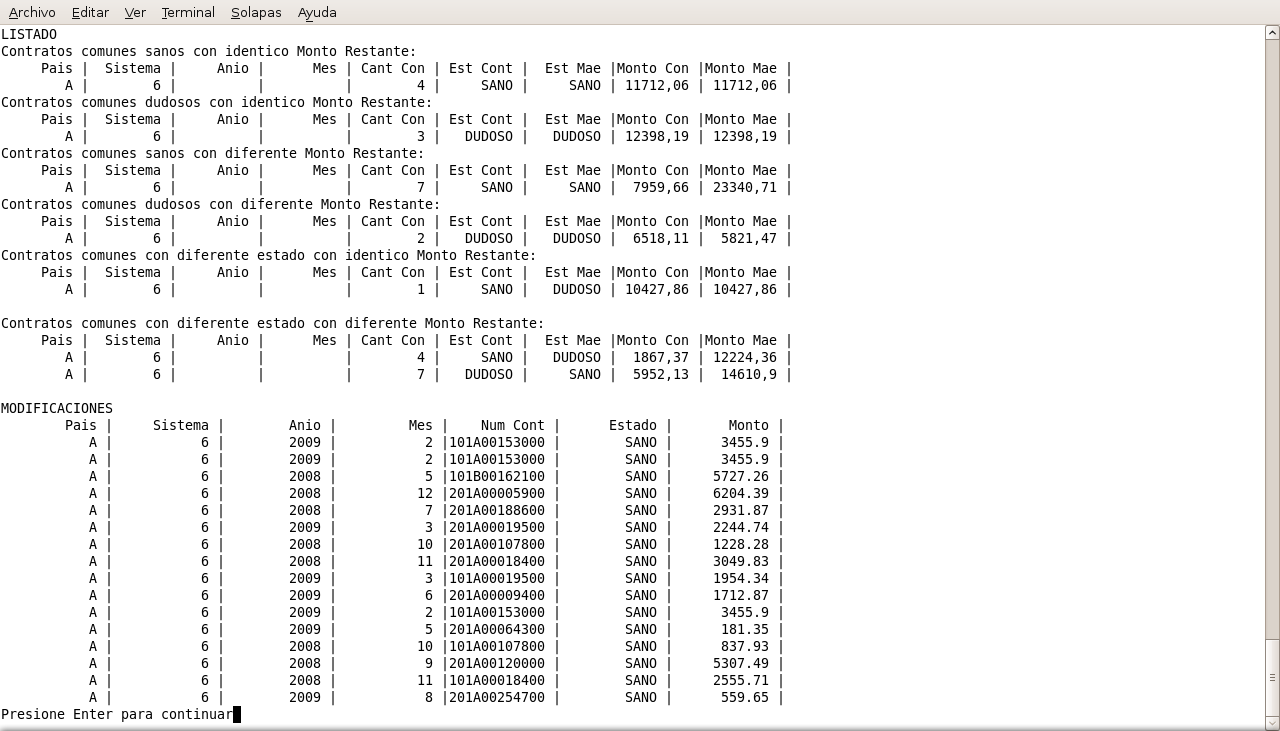
\includegraphics[scale=0.35]{imagenes/reporte/reporte_listadosYModificaciones_A_6.png}
	\caption{Ejemplo consulta}
	\end{figure}

        La siguiente imagém corresponde a la consulta \verb|país: A sistema: 6|.
        No hay restricción sobre el resto de los parámetros.
        La salida de los listados en archivos se produce en 6 ficheros distintos, llamados listadosX.<id>, en donde ``X'' e ``id'' denominan al tipo de consulta y usuario que la realizo, respectivamente. 


	\item [Código fuente:]

\end{description}
{\footnotesize
\verbatiminput{../bin/reporte.pl}
}

\subsection{Comando X}
\begin{description}
	\item [Tipo de comando:] [Solicitado | Auxiliar]
	
	\item [Justificación:] (de su uso si es auxiliar)
	
	\item [Archivos de entrada:]
	
	\item [Archivos de salida:]
	
	\item [Parámetros:] (si tiene)
	
	\item [Opciones:] (si tiene)
	
	\item [Ejemplos de invocación:]
	
	\item [Código fuente:]
\end{description}
% IMPORTANTE: Reemplazar tabulador por 4 espacios en los archivos fuente
{\footnotesize
%\verbatiminput{ruta relativa al archivo fuente}
}

\section{Archivos}
\subsection{Archivo de configuración general}
\begin{description}
	\item [Nombre:] \verb|$GRUPO/practico.conf|
	\item [Estructura:] Este archivo consta de líneas que pueden ser de alguno de los siguientes tipos:
	\begin{itemize}
		\item En blanco
		\item Comentario, comenzando la línea con \verb|#| sin espacios previos
		\item Definición de una variable en formato bash: \verb|VARIABLE=VALOR|. El valor puede contener espacios internos, si debe tener espacios al comienzo deben escapearse o encomillarse, aunque se recomienda especialmente no utilizar espacios en las rutas.
	\end{itemize}
	Este archivo debe tener como mínimo una serie de variables indispensables que el comando instalar generará. Por tal motivo se recomienda que en caso de modificación no se eliminen variables previamente creadas, solo se las modifique y se agreguen variables nuevas.
\end{description}

\subsection{Archivo X}
\begin{description}
	\item [Nombre:] Su nombre
	\item [Estructura:] Descripción de la estructura
	\item [Justificación:] (de su uso si no es requerido por el enunciado)
\end{description}


\end{document}
